\documentclass[12pt]{report}
\usepackage[utf8]{inputenc}
\usepackage{a4}
\usepackage[none]{hyphenat} %hyphenation
\sloppy
\usepackage{parskip} %no indentation after paragraphs
\usepackage{umlaute}
\usepackage{afterpage} %for using \afterpage{\clearpage} (don't push images to the end of a chapter)
\usepackage{makeidx}
\usepackage[numbers]{natbib}
\usepackage{picins} %provides precise control over the placement of inline graphics
\usepackage{setspace}
\usepackage{titlesec}
\usepackage{dsfont} %math symbols
\usepackage{tabularx}
\usepackage{floatflt} %float text around figures and tables
\usepackage{enumitem} %resume counting from previous enumerate block
\usepackage{amsmath,amssymb}
\usepackage[format=default,font=footnotesize,labelfont=bf]{caption}
\usepackage{listings} %for listing source code
\usepackage{color}
\usepackage{float} % for [H] after floats
\usepackage{url}
\usepackage{graphicx} 
\usepackage{todonotes}
\usepackage[automake]{glossaries}
\newglossary[slg]{symbolslist}{syi}{syg}{Symbols}
\makeglossaries
\newacronym{TUM}{TUM}{Technical University Munich}
\newacronym{UI}{UI}{User Interface}
\newacronym{IDP}{IDP}{Interdisciplinary Project}
\newacronym{URL}{URL}{Uniform Resource Locator}
\newacronym{JSON}{JSON}{Javascript Object Notation}
\newacronym{HTTP}{HTTP}{Hypertext Transfer Protocol}
\newacronym{API}{API}{Application Programming Interface}
\newacronym{VM}{VM}{Virtual Machine}
\newacronym{SHA}{SHA}{Secure Hash Algorithm}
\newacronym{RSA}{RSA}{Rivest–Shamir–Adleman Algorithm}
\newacronym{PoW}{PoW}{Proof of Work}
\newacronym{LRZ}{LRZ}{Leibniz-Rechenzentrum}
\newacronym{CSV}{CSV}{Comma-Separated Values}
\newacronym{XML}{XML}{Extensible Markup Language}
\newacronym{GUI}{GUI}{Graphical User Interface}
\newacronym{SSH}{SSH}{Secure SHell}
\newacronym{DLT}{DLT}{Distributed Ledger Technology}
\newacronym{DAG}{DAG}{Directed Acyclic Graph}



\newglossaryentry{Blockchain}{
	name={Blockchain},
    description={ A blockchain, originally block chain, is a continuously growing list of records, called blocks, which are linked and secured using cryptography. Each block typically contains a hash pointer as a link to a previous block, a timestamp and transaction data},
    first = {Blockchain},
}

\newglossaryentry{Cryptography}{
	name={Cryptography},
    description={ Cryptography is the practice and study of techniques for secure communication in the presence of third parties called adversaries},
    first = {cryptography},
}

\newglossaryentry{publickey}{
	name={Public Key},
    description={ In cryptography, a public key is a value provided by some designated authority as an encryption key that, combined with a private key derived from the public key, can be used to effectively encrypt messages and digital signatures},
    first = {public key},
}

\newglossaryentry{Cryptocurrency}{
	name={Cryptocurrency},
    description={ A cryptocurrency (or crypto currency) is a digital asset designed to work as a medium of exchange that uses cryptography to secure its transactions, to control the creation of additional units, and to verify the transfer of assets},
    plural = {cryptocurrencies},
}

\newglossaryentry{REST}{
	name={REST},
    description={An acronym for Representational State Transfer, is a common architectural pattern for web applications},
    first = {Representational State Transfer(REST)},
}

\newglossaryentry{nonce}{
	name={nonce},
    description={In cryptography, a nonce is an arbitrary number that can only be used once. It is similar in spirit to a nonce word, hence the name. It is often a random or pseudo-random number issued in an authentication protocol to ensure that old communications cannot be reused in replay attacks},
}

\newglossaryentry{electron}{
	name={Electron},
    description={Electron (formerly known as Atom Shell) is an open-source framework created by Cheng Zhao, and now developed by GitHub. It allows for the development of desktop GUI applications using front and back end components originally developed for web applications: Node.js runtime for the backend and Chromium for the frontend},
}


\newglossaryentry{encryption key}{
	name={Encryption Key},
    description={A string of binary digits used by cryptographic algorithms used in encrypting and decrypting information},
    plural = {encryption keys},
}

\newglossaryentry{Docker}{
	name={Docker},
    description={ Docker is an open platform for developers and sysadmins to build, ship, and run distributed applications, whether on laptops, data center VMs, or the cloud},
    first = {Docker},
}

\newglossaryentry{hash}{
	name={Hash Function},
    description={ A hash function is any function that can be used to map data of arbitrary size to data of fixed size. The values returned by a hash function are called hash values, hash codes, digests, or simply hashes.},
    first = {hash},
}



\newglossaryentry{Bitcoin}{
	name={Bitcoin},
    description={Bitcoin is a cryptocurrency and worldwide payment system. It is the first decentralized digital currency, as the system works without a central bank or single administrator. The network is peer-to-peer and transactions take place between users directly, without an intermediary},
    first = {Bitcoin},
} % all abbreviations
\newglossaryentry{symb:N}{sort={3},
name={$\mathbb N$},
first={first $\mathbb N$},
text={additional $\mathbb N$},
description={Set of natural numbers},
type=symbolslist} % all symbols
\glsaddall[types=\acronymtype]
\usepackage{listings}
\usepackage{color}
\definecolor{gray}{rgb}{0.4,0.4,0.4}
\definecolor{darkblue}{rgb}{0.0,0.0,0.6}
\definecolor{cyan}{rgb}{0.0,0.6,0.6}
\usepackage[autostyle]{csquotes}
\usepackage{subcaption}
\usepackage[ruled,lined,linesnumbered, noend]{algorithm2e}
\usepackage{algorithmicx}
\usepackage{algpseudocode}
\usepackage[]{algorithm2e}
\usepackage{multirow}
\usepackage{rotating}
\usepackage[toc,page]{appendix}
\usepackage{CJKutf8}
\usepackage{longtable}


\setlength{\extrarowheight}{10pt}

\lstset{
	basicstyle=\ttfamily,
	columns=fullflexible,
	showstringspaces=false,
	commentstyle=\color{gray}\upshape
}

\titleformat{\paragraph}[hang]{\normalfont\bfseries}{\theparagraph}{.5em}{}

\makeindex
\frenchspacing
\sloppy
\pagestyle{headings}
\textwidth16cm
\textheight22cm
\topmargin0cm
\oddsidemargin0cm
\evensidemargin0cm

\newcommand\tab[1][1cm]{\hspace*{#1}}

\newcommand{\bildklein}[3]{  
	\begin{figure}[hp]
	\begin{center}
	\includegraphics[width=0.5\textwidth]{#1}
	\end{center}
	\caption[#2]{#3}
	\end{figure}
}	
\newcommand{\bildgross}[3]{  
	\begin{figure}[hp]
	\begin{center}
	\includegraphics[width=0.95\textwidth]{#1}
	\end{center}
	\caption[#2]{#3}
	\end{figure}
}

% This is tumlogo.tex
%
% Neues TUM-Logo in TeX
%   by G. Teege, 19.10.89
% Benutzung:
%   Am Anfang des Dokuments (TeX oder LaTeX):
%     \input tumlogo
%   Dann beliebig oft:
%     \TUM{<breite>}
%   bzw.
%     \oTUM{<breite>}
%   \TUM setzt das Logo mit der Breite <breite> und der entsprechenden Hoehe.
%   <breite> muss eine <dimen> sein. \oTUM erzeugt eine "outline"-Version
%   des Logos, d.h. weiss mit schwarzem Rand. Bei \TUM ist es ganz schwarz.
%   \oTUM entspricht damit der offiziellen Version des Logos.
%   Das Logo kann wie ein einzelnes Zeichen verwendet werden.
%   Beispiel:
%     Dies ist das TUM-Logo: \oTUM{1cm}.
%
\def\TUM#1{%
\dimen1=#1\dimen1=.1143\dimen1%
\dimen2=#1\dimen2=.419\dimen2%
\dimen3=#1\dimen3=.0857\dimen3%
\dimen4=\dimen1\advance\dimen4 by\dimen2%
\setbox0=\vbox{\hrule width\dimen3 height\dimen1 depth0pt\vskip\dimen2}%
\setbox1=\vbox{\hrule width\dimen1 height\dimen4 depth0pt}%
\setbox2=\vbox{\hrule width\dimen3 height\dimen1 depth0pt}%
\setbox3=\hbox{\copy0\copy1\copy0\copy1\box2\copy1\copy0\copy1\box0\box1}%
\leavevmode\vbox{\box3}}
%
\def\oTUM#1{%
\dimen1=#1\dimen1=.1143\dimen1%
\dimen2=#1\dimen2=.419\dimen2%
\dimen3=#1\dimen3=.0857\dimen3%
\dimen0=#1\dimen0=.018\dimen0%
\dimen4=\dimen1\advance\dimen4 by-\dimen0%
\setbox1=\vbox{\hrule width\dimen0 height\dimen4 depth0pt}%
\advance\dimen4 by\dimen2%
\setbox8=\vbox{\hrule width\dimen0 height\dimen4 depth0pt}%
\advance\dimen4 by-\dimen2\advance\dimen4 by-\dimen0%
\setbox4=\vbox{\hrule width\dimen4 height\dimen0 depth0pt}%
\advance\dimen4 by\dimen1\advance\dimen4 by\dimen3%
\setbox6=\vbox{\hrule width\dimen4 height\dimen0 depth0pt}%
\advance\dimen4 by\dimen3\advance\dimen4 by\dimen0%
\setbox9=\vbox{\hrule width\dimen4 height\dimen0 depth0pt}%
\advance\dimen4 by\dimen1%
\setbox7=\vbox{\hrule width\dimen4 height\dimen0 depth0pt}%
\dimen4=\dimen3%
\setbox5=\vbox{\hrule width\dimen4 height\dimen0 depth0pt}%
\advance\dimen4 by-\dimen0%
\setbox2=\vbox{\hrule width\dimen4 height\dimen0 depth0pt}%
\dimen4=\dimen2\advance\dimen4 by\dimen0%
\setbox3=\vbox{\hrule width\dimen0 height\dimen4 depth0pt}%
\setbox0=\vbox{\hbox{\box9\lower\dimen2\copy3\lower\dimen2\copy5%
\lower\dimen2\copy3\box7}\kern-\dimen2\nointerlineskip%
\hbox{\raise\dimen2\box1\raise\dimen2\box2\copy3\copy4\copy3%
\raise\dimen2\copy5\copy3\box6\copy3\raise\dimen2\copy5\copy3\copy4\copy3%
\raise\dimen2\box5\box3\box4\box8}}%
\leavevmode\box0}
% End of tumlogo.tex



\begin{document}

\hoffset=5mm
\thispagestyle{empty}
\begin{center}
	\bigskip \bigskip \bigskip 
	\oTUM{6.0cm} \\
	\vspace*{0.8cm}
	{\huge \bf Technische Universität} \\
	\bigskip
	{\huge \bf München} \\
	\bigskip \bigskip \bigskip
	{\huge \bf Fakultät für Informatik} \\
	\bigskip \bigskip \bigskip
	{\Large \bf Master's Thesis in Informatik} \\
	\bigskip \bigskip \bigskip \bigskip \bigskip
	{\Large  Design and Implementation of a Simulation Framework for Blockchain Alternatives: A Directed Acyclic Graph Based Distributed Ledger} \\        
	\bigskip \bigskip \bigskip \bigskip
	{\Large Mohamed Riswan Abdul Lathif} \\    
	\bigskip
	\begin{figure}[ht]
	\centering 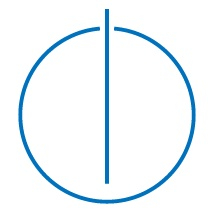
\includegraphics[width=0.2\linewidth]{figures/infologo.jpg}
	\end{figure}
	\bigskip 
\end{center}
\vfill

\newpage
\hoffset=5mm
\thispagestyle{empty}
\begin{center}
	\bigskip \bigskip \bigskip 
	\oTUM{6.0cm} \\
	\vspace*{0.8cm}
	{\huge \bf Technische Universität} \\
	\bigskip
	{\huge \bf München} \\
	\bigskip \bigskip \bigskip
	{\huge \bf Fakultät für Informatik} \\
	\bigskip \bigskip \bigskip
	{\Large \bf Master's Thesis in Informatik} \\
	\bigskip \bigskip \bigskip \bigskip \bigskip
	{\Large Design and Implementation of a Simulation Framework for Blockchain Alternatives: A Directed Acyclic Graph Based Distributed Ledger} \\
	\bigskip \bigskip \bigskip
	{\Large Gestaltung und Umsetzung eines Simulationsframeworks für Blockchain Alternativen: 
Ein Distributed Ledger System basierend auf gerichteten azyklischen Graphen} \\
	\bigskip
\end{center}
\vfill
\begin{tabular}{ll}
{\Large \bf Author:} & {\Large Mohamed Riswan Abdul Lathif} \\\\
{\Large \bf Supervisor:} & {\Large Prof. Dr. Hans-Arno Jacobsen} \\\\
{\Large \bf Advisor:} & {\Large Pezhman Nasirifard} \\\\
{\Large \bf Submission:} & {\Large 14.01.2019}
\end{tabular}

\newpage	
\thispagestyle{empty}
\hoffset=0mm
\vspace*{\fill}
\noindent I confirm that this master's thesis is my own work and I have documented all sources and material used.\\\\
München, 14.01.2019\\\\\\\\\\\\
\noindent \textit{(Mohamed Riswan Abdul Lathif)}

\newpage
\thispagestyle{empty}
\null

\newpage
\thispagestyle{empty}
\hoffset=0mm
\section*{Abstract}	
\begin{spacing}{1.2}
Blockchain basierte Distributed Ledgers gehören in der heutigen Zeit zu den größten Forschungsfeldern. Die Gründe liegen hier besonders in den Erfolgen von Kryptowährungen wie Bitcoin, Etherium, usw. Trotz vieler Vorteile sind Blockchain Systeme meist ressourcenintensiv und schwer skalierbar. Daher suchen viele Wissenschaftler nach Alternativen für Blockchain Systeme. Eine dieser Alternativen ist Tangle, welches von der IOTA Stiftung ins Leben gerufen wurde. Tangle ist ein auf gerichteten zyklischen Graphen (Directed Acyclic Graph oder DAG) basierendes Distributed Ledger System, welches Vorteile wie etwa hohe Skalierbarkeit oder Unterstützung für Micropayments fördert. Außerhalb des Kontextes der IOTA Stiftung wurden die Eigenschaften von DAG basierten Distributed Ledger Systemen allerdings noch nicht erforscht. Des Weiteren enthält IOTA bislang noch keine großen Peer-To-Peer Simulationssysteme mit anpassbaren Parametern, welche den Nutzern das Erforschen von wichtigen Charakteristiken bzw. Metriken des Netzwerks und das Vergleichen von verschiedenen Situationen in kontrollierten Bedingungen ermöglicht. Als Lösung dieses Problems schlagen wir CIDDS, ein konfigurierbares und interaktives DAG basiertes Distributed Ledger Simulationssystem (eng. Configurable and Interactive DAG Based Distributed Ledger Simulations Framework), vor . Mit CIDDS können Nutzer eine große skalierbare Simulation mit tausenden von Knoten erstellen und die Eigenschaften der entstandenen DAG Ledgers mit unterschiedlichen Parametern erforschen.
\end{spacing}
 
\newpage
\thispagestyle{empty}
\hoffset=0mm
\section*{Inhaltsangabe}
\begin{spacing}{1.2}
Blockchain based distributed ledgers is one of the most studied research areas, owing to the enormous success of crypto-currencies like Bitcoin, Etherium, etc. But, in addition to all the advantages, Blockchain is by design resource intensive and in general does not scale well. Hence, researchers all over are looking for alternatives for blockchain and one such alternative is the Tangle, introduced by IOTA foundation. Tangle is a Directed Acyclic Graph (DAG) based distributed ledger, which boasts advantages like high scalability and support for micro-payments. But outside the context of IOTA, the properties of a DAG-based distributed ledger are not studied. Also IOTA currently does not contain a large scale peer-to-peer simulation system with configurable parameters, which allows the users to study the important characteristics and metrics of the network and compare different scenarios under controlled conditions. This thesis proposes CIDDS, a Configurable and Interactive DAG based Distributed ledger Simulation framework as a solution to this problem. Using CIDDS, users can create large scale tangle simulations with thousands of nodes and study the characteristics of the resulting DAG ledgers with varying parameters.
\end{spacing}

\newpage
\thispagestyle{empty}
\hoffset=0mm
\section*{Acknowledgment}	
\begin{spacing}{1.2}
I would like to extend my sincere thanks to my advisor Pezhman Nasirifard for being the best advisor possible and helping me out with all the issues I faced. I would also like to express my gratitude for my supervisor Prof. Dr. Hans-Arno Jaconbsen for providing me an opportunity to write this thesis at his chair at TU Munich and for the constant inspiration.

I would also like to thank Alon Gal from the IOTA foundation for his valuable inputs in designing this simulator. Also I express my gratitude to Minh-Nghia Nguyen for his correspondence and input in implementation of the tip selection algorithms used in the simulator.
\end{spacing}

\newpage
\setcounter{page}{1}
\hoffset=0mm
\fboxsep 0mm

\tableofcontents
\setcounter{tocdepth}{2}

\listoffigures
\addcontentsline{toc}{chapter}{List of Figures}

\listoftables
\addcontentsline{toc}{chapter}{List of Tables}

\printglossary[type=\acronymtype,style=long ,title=Abbreviations, toctitle=Abbreviations,nonumberlist]
\printglossary[type=symbolslist,style=long ,title=Symbols, nonumberlist]
\addcontentsline{toc}{chapter}{Abbreviations}

\newpage
\setlength{\baselineskip}{3ex}
\begin{spacing}{1.15}
\chapter{Introduction} 
\label{chapter:introduction}

\gls{Blockchain} based distributed ledgers have taken the computing world by storm and the huge success of Bitcoin and other \glspl{Cryptocurrency} has sparked an academic interest over the \gls{DLT}. Unfortunately, Blockchain based DLTs also have major disadvantages which cannot be overlooked and hence extensive research towards alternatives for Blockchain based \gls{DLT}s is needed. One such alternative is the \gls{DAG} based \gls{DLT}. \\

\gls{DAG} based DLTs have gained prominence with the introduction of IOTA and the Tangle introduced in \cite{Tangle} outlined the possibility of having a DLT which can scale infitely, atleast in theory.

\section{Motivation} 
\label{sec:motivation}

Motivation of Thesis.

\section{Problem Statement} 
\label{sec:problemStatement}

Problem Statement of Thesis.

\section{Approach}
 \label{sec:approach}

Your Approach overview.

\section{Organization}
 \label{sec:organization}

Organization of Thesis.
\chapter{Background} 
\label{chapter:background}

Background concepts required for understanding the thesis. 
\chapter{Related Work}
\label{chapter:relatedWork}

Related work materials 

\chapter{Approach}\label{chapter:approach}
Approach

\section{Prerequisites}
Approach \gls{SA}

\section{Design of Proposed Solution}

\subsection{Architecture}


\section{Implementation}

\subsection{Technology Choice}

\subsection{Frontend}


\chapter{Evaluation}
\label{chapter:evaluation}

The evaluation chapter.

\chapter{Summary} \label{chapter:summary}

Summary

\section{Status} 
\label{sec:status}

Final Status of the Thesis

\section{Conclusions}
\label{sec:conclusions}

Concluding remarks of Thesis

\section{Future Work} 
\label{sec:futureWork}

Future Work
\end{spacing}

\newpage
\begin{appendices}
\addtocontents{toc}{\protect\setcounter{tocdepth}{0}}
\chapter{Appendix}

\section{First}

First Appendix

\end{appendices}

\newpage
\bibliographystyle{IEEEtran}
\bibliography{IEEEabrv,literature}
\end{document}